\section{Introduction}
Parkinson's disease is a progressive neurodegenerative disorder; more than 8.5 million people were living with PD worldwide in 2019, and disability and death due to PD are rising faster than for any other neurological disorder [1]. Diagnosis remains largely clinical and is usually prompted by motor signs such as tremor, rigidity and slowness of movement, by which point substantial neuronal loss has already occurred.

Speech offers an earlier and more accessible signal. An estimated 89\% of people with PD develop a speech or voice disorder, with reduced loudness, monotone pitch, breathiness and imprecise articulation [2], and voice has been reported as the leading and earliest-affected speech dimension [3]. Because these changes are gradual, patients rarely notice them; an objective, low-cost measurement taken from a sustained vowel is therefore attractive as a first-line screen.

This work contributes (i) a two-branch classifier that combines interpretable Praat acoustic measures with a transfer-learned spectrogram model, (ii) an agreement-based ensemble policy that trades sensitivity for precision in an explicit and analysable way, (iii) an end-to-end deployment path that accepts audio from a browser or an ordinary telephone call, and (iv) a reproducible characterisation of the acoustic front-end on controlled synthetic phonation. The paper deliberately separates what is measured from what is designed, and does not report unverified accuracy figures.

\section{Related Work}
Little et al.\ showed that dysphonia measures computed from sustained phonation---jitter, shimmer, noise-to-harmonics ratios and nonlinear recurrence and fractal-scaling measures---separate PD from healthy speakers, and released the Oxford Parkinson's Disease Detection dataset of 195 recordings from 31 speakers, 23 with PD [4], [5]. This dataset has become the standard benchmark for speech-based PD detection. Sakar et al.\ collected a richer corpus with multiple recording types per subject and evaluated a range of classifiers [6]; across the literature, Support Vector Machines, k-nearest neighbours and tree ensembles such as Random Forest and gradient boosting are consistently competitive on these tabular features.

A second strand treats detection as image classification on spectrograms using convolutional networks and, more recently, transformers. The Vision Transformer of Dosovitskiy et al.\ splits an image into 16$\times$16 patches processed by a standard Transformer encoder and transfers well from large-scale pretraining [7]. The present system builds on both strands and uses Praat [10] through the Parselmouth Python interface [8], scikit-learn [9] and PyTorch.

\section{System Architecture}
The system is an audio-in, probability-out pipeline (Fig.~1). Audio arrives either from a browser upload or from a Twilio voice call. An ingestion stage converts MP3 and WMA input to mono WAV using pydub with an ffmpeg backend. The waveform is then processed by two independent branches: an acoustic-feature branch that feeds a Random Forest, and a spectrogram branch that feeds a Vision Transformer. Both outputs are combined in a single \texttt{classify()} interface used by every entry point. Each stage emits a well-defined artefact---a WAV file, a feature vector, a spectrogram image, a probability---so the stages can be developed and tested independently.

\begin{figure}[!t]
\centering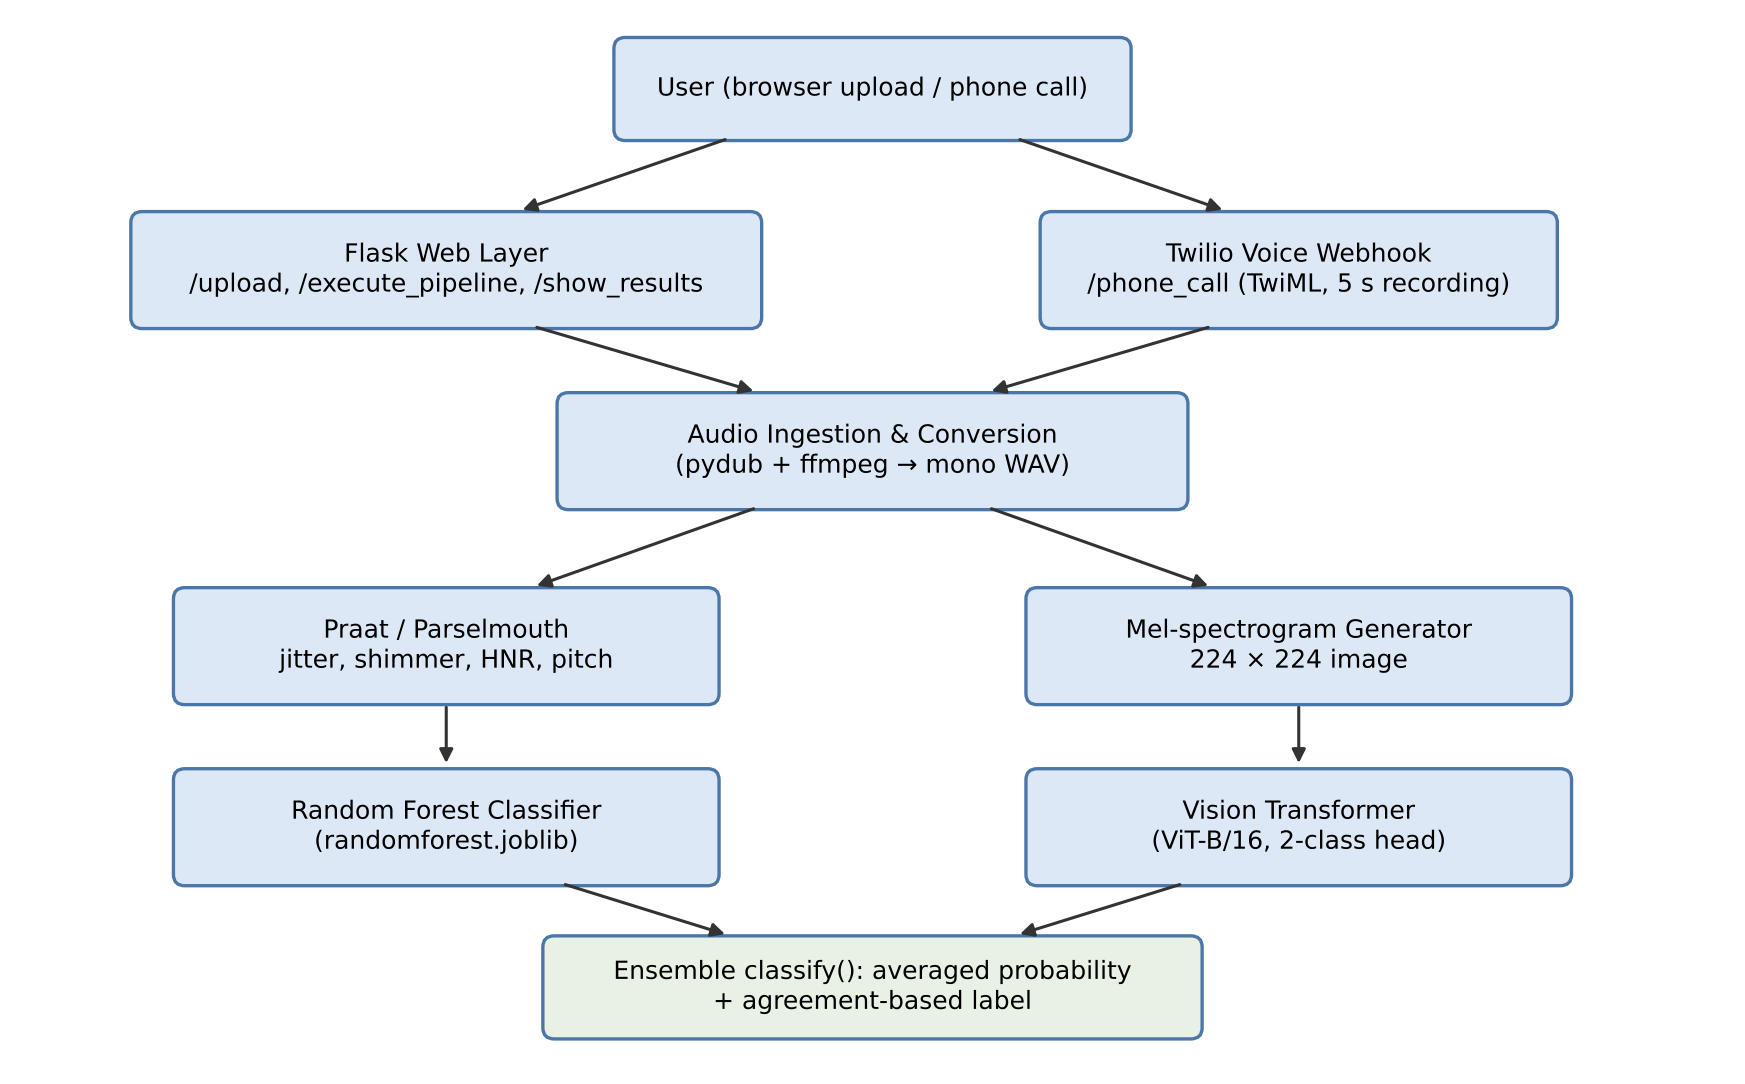
\includegraphics[width=\columnwidth]{figs/pk_fig1.png}
\caption{Logical architecture of the screening system.}
\end{figure}

\section{Methodology}
\subsection{Acoustic Feature Extraction}
Parselmouth constructs a periodic point process from each recording (pitch floor 75~Hz, ceiling 500~Hz) and computes a fixed feature vector: jitter (local, absolute, RAP, PPQ5, DDP), shimmer (local, dB, APQ3, APQ5, APQ11, DDA), mean HNR and mean fundamental frequency. Local jitter is the mean absolute difference between consecutive glottal periods divided by the mean period; local shimmer is the analogous quantity for peak amplitudes. Both increase when phonation becomes irregular, while HNR decreases as aspiration noise increases. The vector is summarised in Table~I.

\begin{table}[!t]
\caption{Acoustic Feature Vector Used by the Random Forest}
\centering\footnotesize
\begin{tabularx}{\columnwidth}{@{}l>{\raggedright\arraybackslash}X>{\raggedright\arraybackslash}X@{}}
\toprule
\textbf{Group} & \textbf{Measures} & \textbf{Captures}\\\midrule
Jitter & local, absolute, RAP, PPQ5, DDP & Cycle-to-cycle period instability\\
Shimmer & local, dB, APQ3, APQ5, APQ11, DDA & Cycle-to-cycle amplitude instability\\
Noise & mean HNR & Breathiness / aspiration noise\\
Pitch & mean F0 & Speaker baseline; monotone tendency\\\bottomrule
\end{tabularx}
\end{table}

\subsection{Random Forest Branch}
A Random Forest is trained on the feature vectors with scikit-learn, its hyper-parameters are selected by cross-validation, and the fitted model is persisted with joblib (approximately 2.6~MB). Because it is small and CPU-only, it is the always-available decision model in every deployment. Recordings from the same speaker must be kept within one fold to avoid optimistic leakage.

\subsection{Vision Transformer Branch}
A mel-spectrogram is generated for each sample, resized to 224$\times$224 and passed to ViT-B/16 pretrained on ImageNet. The image yields 196 non-overlapping 16$\times$16 patches plus a class token; the encoder (12 layers, hidden size 768) is frozen and only a replacement linear head of 768$\times$2 weights plus 2 biases (1,538 parameters) is trained with a Softmax output. Freezing the body keeps training tractable on modest hardware and limits over-fitting on small corpora.

\subsection{Agreement Ensemble}
Let $p_{\mathrm{RF}}$ and $p_{\mathrm{ViT}}$ be the two PD probabilities. The reported confidence is their mean, but the label is positive only when both models individually predict PD; otherwise the sample is reported as healthy. If the two classifiers have sensitivities $Se_1, Se_2$ and specificities $Sp_1, Sp_2$ and their errors are conditionally independent given the true class, the agreement rule yields
\begin{equation}
Se_{\mathrm{AND}} = Se_1 Se_2,\qquad Sp_{\mathrm{AND}} = 1-(1-Sp_1)(1-Sp_2).
\end{equation}
The rule therefore multiplies false-positive rates while also multiplying sensitivities: it is a deliberate precision-for-recall trade. Positive correlation between the models' errors weakens the specificity gain, which is why two model families with different inductive biases are combined.

\section{Implementation and Deployment}
The web layer is a Flask application whose Jinja templates render index, loading and results pages and whose endpoints are \texttt{/upload}, \texttt{/execute\_pipeline} and \texttt{/show\_results}. A separate \texttt{/phone\_call} endpoint returns TwiML that prompts the caller to sustain ``aaaa'', records five seconds, downloads the recording and speaks the classification back. The application runs under gunicorn; an Aptfile pins ffmpeg, a Dockerfile provides a self-contained image and a \texttt{render.yaml} blueprint enables one-click hosting on a free tier. Twilio credentials are read from environment variables rather than source code.

\section{Numerical Analysis}
\subsection{Front-End Sensitivity on Controlled Synthetic Vowels}
To verify that the feature branch responds to the perturbations it is meant to detect, sustained vowels were synthesised at 16~kHz with a 125~Hz fundamental (an integer 128-sample period, eliminating quantisation jitter) by exciting three damped formant resonators (700, 1220 and 2600~Hz) with a pulse train. Gaussian period perturbation, amplitude perturbation or additive noise was injected one factor at a time, and each condition was averaged over five random seeds of 3~s each. All values in Tables~II--III were measured with Parselmouth 0.4.7 and are reproducible from the stated generator.

\begin{table}[!t]
\caption{Measured Response to Injected Period Perturbation}
\centering\footnotesize
\begin{tabular}{@{}cccc@{}}\toprule
\textbf{Injected $\sigma$ (\%)} & \textbf{Jitter local (\%)} & \textbf{Shimmer local (\%)} & \textbf{HNR (dB)}\\\midrule
0.00 & 0.000 & 0.002 & 74.6\\
0.25 & 0.389 & 0.526 & 41.1\\
0.50 & 0.653 & 0.837 & 25.0\\
1.00 & 1.171 & 1.174 & 15.1\\
1.50 & 1.705 & 1.312 & 11.3\\
2.00 & 2.287 & 1.475 & 9.1\\\bottomrule
\end{tabular}
\end{table}

Measured jitter rises monotonically with the injected perturbation (Fig.~2, left), from 0.000\% for a perfectly periodic source to 2.287\% at $\sigma = 2\%$, and mean HNR falls from 74.6~dB to 9.1~dB because cycle-to-cycle irregularity spreads energy between harmonics. Shimmer responds to amplitude perturbation almost one-to-one (Fig.~2, right) while measured jitter stays below 0.025\%, confirming that the two measures are largely separable.

\begin{figure}[!t]
\centering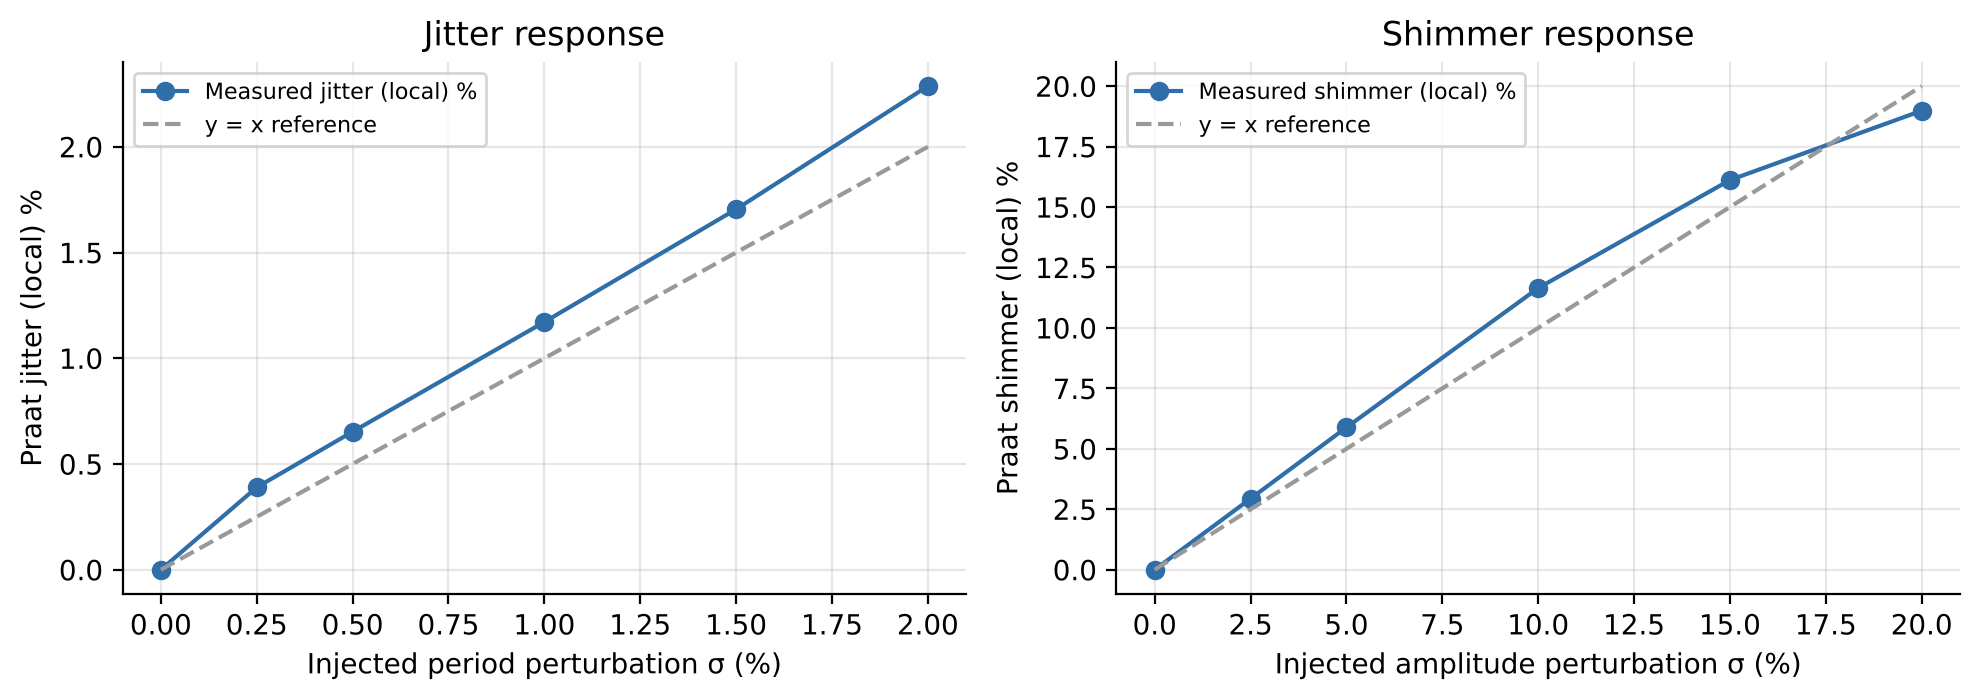
\includegraphics[width=\columnwidth]{figs/pk_fig2.png}
\caption{Praat jitter and shimmer versus injected perturbation (synthetic vowels, mean of five seeds).}
\end{figure}

\begin{table}[!t]
\caption{Measured Response to Additive Noise}
\centering\footnotesize
\begin{tabular}{@{}ccc@{}}\toprule
\textbf{Noise level} & \textbf{Shimmer local (\%)} & \textbf{HNR (dB)}\\\midrule
0.01 & 0.598 & 27.3\\
0.02 & 1.195 & 21.2\\
0.05 & 2.959 & 13.3\\
0.10 & 5.731 & 7.3\\
0.20 & 9.998 & 1.3\\\bottomrule
\end{tabular}
\end{table}

Additive noise lowers HNR from 27.3~dB to 1.3~dB across the tested range, and also inflates measured shimmer to 10.00\% at the highest level. This coupling is practically important: telephone-channel noise can mimic pathological shimmer, so a model trained on clean recordings may over-call PD on noisy calls---one reason the conservative ensemble rule is adopted. Fig.~3 shows the corresponding change in the time-domain waveform and in the mel-spectrogram that the ViT branch receives: the harmonic striations that dominate the stable vowel become blurred and the inter-harmonic floor rises.

\begin{figure}[!t]
\centering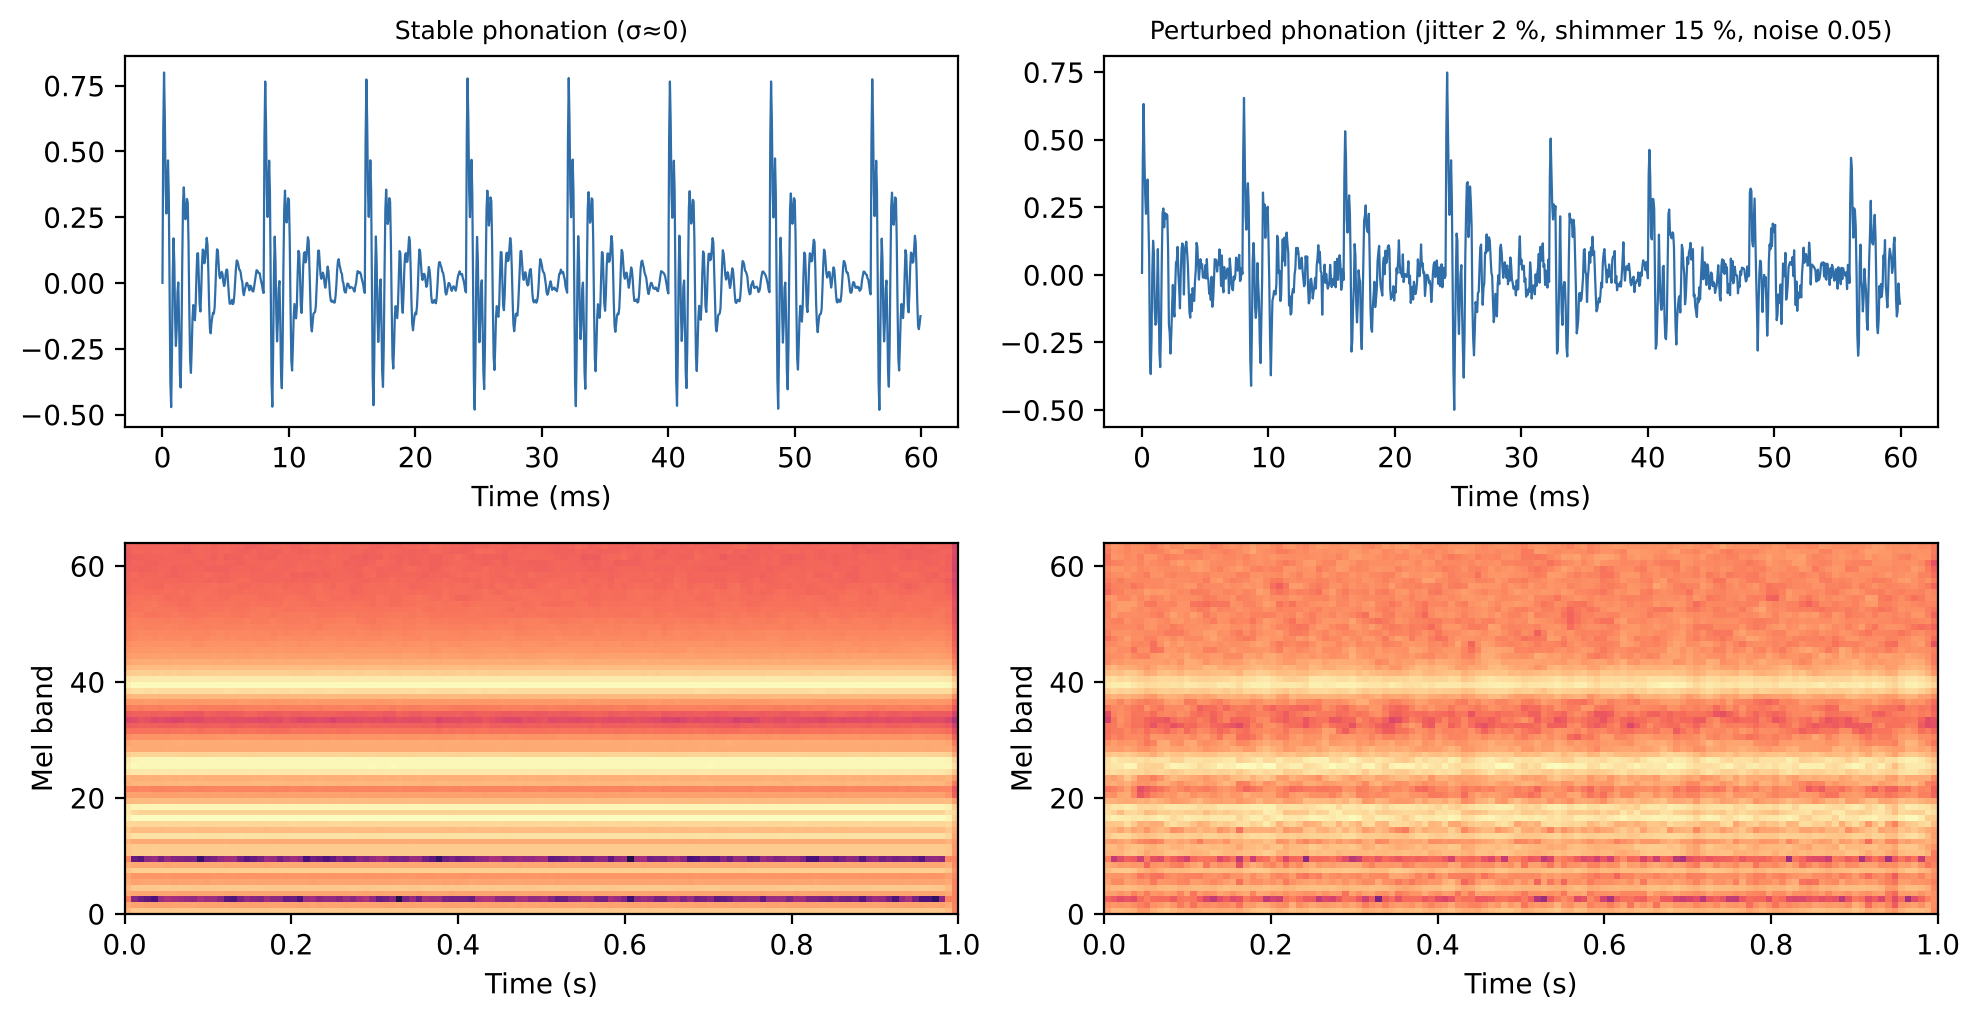
\includegraphics[width=\columnwidth]{figs/pk_fig3.png}
\caption{Synthetic stable and perturbed vowels: waveform (top) and mel-spectrogram (bottom).}
\end{figure}

\subsection{Agreement-Rule Analysis}
Table~IV applies (1) to illustrative, assumed operating points ($Se_1=0.90$, $Sp_1=0.80$; $Se_2=0.85$, $Sp_2=0.75$). These are not measured accuracies; they show the shape of the trade-off only.

\begin{table}[!t]
\caption{Illustrative Effect of the Ensemble Rule (Assumed Inputs)}
\centering\footnotesize
\begin{tabular}{@{}lccc@{}}\toprule
\textbf{Rule} & \textbf{Sensitivity} & \textbf{Specificity} & \textbf{PPV, prev.\ 1\%}\\\midrule
RF alone & 0.900 & 0.800 & 0.043\\
ViT alone & 0.850 & 0.750 & 0.033\\
AND (agreement) & 0.765 & 0.950 & 0.134\\
OR (either) & 0.985 & 0.600 & 0.024\\\bottomrule
\end{tabular}
\end{table}

\begin{figure}[!t]
\centering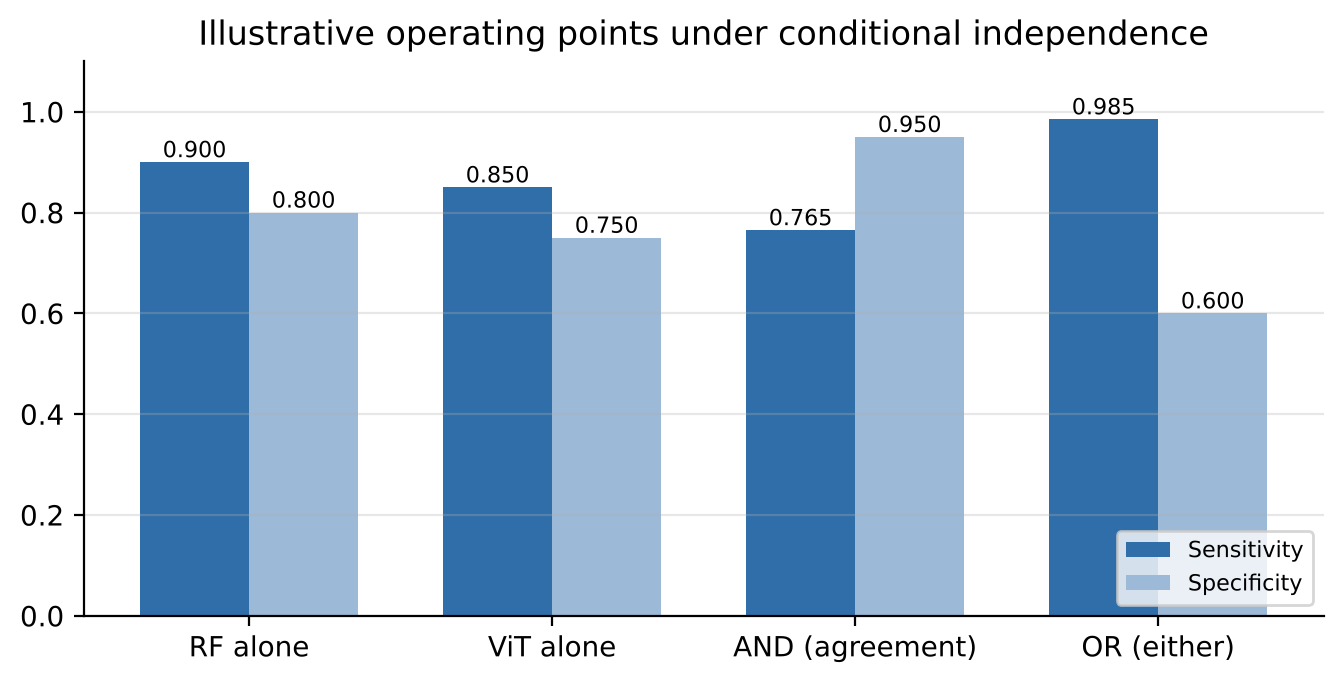
\includegraphics[width=\columnwidth]{figs/pk_fig4.png}
\caption{Sensitivity and specificity of single models and combination rules under conditional independence (assumed inputs).}
\end{figure}

At a screening prevalence of 1\%, the agreement rule raises positive predictive value from 0.03--0.04 for either model alone to 0.134, at the cost of reducing sensitivity to 0.765. For a public, self-administered tool where a false alarm causes anxiety and an unnecessary visit, this direction of trade-off is defensible, but the threshold should ultimately be calibrated on held-out data rather than fixed by a binary rule.

\section{Evaluation Protocol and Threats to Validity}
Classifier accuracy is not reported here because a speaker-independent held-out evaluation was not re-executed for this paper. The required protocol is grouped (speaker-level) cross-validation on the 195-recording corpus, whose 147 PD and 48 healthy recordings give a majority-class baseline of 75.4\% accuracy that any model must clearly beat; per-model and ensemble accuracy, precision, recall, F1 and ROC-AUC with confusion matrices; and a separate test on telephone-band audio. Threats include the small number of speakers, sustained-vowel-only English data, recording-condition mismatch between laboratory and telephone audio, and the conditional-independence assumption behind (1).

\section{Conclusion}
The work delivers a deployable, accessible path from a raw sustained vowel---uploaded or spoken over the phone---to a probability score, combining interpretable Praat measures with a transfer-learned spectrogram model under a conservative agreement policy. Controlled measurements confirm that the acoustic front-end responds monotonically and separably to period, amplitude and noise perturbations, and expose a noise-to-shimmer coupling that motivates channel-aware training. Future work will report speaker-independent accuracy, calibrate the decision threshold, add connected-speech and multilingual data, and validate prospectively against clinician-labelled recordings. The system is intended as a screening aid only and must not be used as a clinical diagnosis.

\section*{References}
{\footnotesize\raggedright
\begin{enumerate}[label={[\arabic*]},leftmargin=2.2em,itemsep=1pt]
\item World Health Organization, ``Parkinson disease,'' Fact sheet, 2023. \url{https://www.who.int/news-room/fact-sheets/detail/parkinson-disease}
\item M. Trail, C. Fox, L. O. Ramig, S. Sapir, J. Howard and E. C. Lai, ``Speech treatment for Parkinson's disease,'' \textit{NeuroRehabilitation}, vol.~20, no.~3, pp.~205--221, 2005.
\item A. K. Ho, R. Iansek, C. Marigliani, J. L. Bradshaw and S. Gates, ``Speech impairment in a large sample of patients with Parkinson's disease,'' \textit{Behavioural Neurology}, vol.~11, no.~3, pp.~131--137, 1998.
\item M. A. Little, P. E. McSharry, E. J. Hunter, J. Spielman and L. O. Ramig, ``Suitability of dysphonia measurements for telemonitoring of Parkinson's disease,'' \textit{IEEE Trans. Biomed. Eng.}, vol.~56, no.~4, pp.~1015--1022, 2009.
\item M. A. Little, P. E. McSharry, S. J. Roberts, D. A. E. Costello and I. M. Moroz, ``Exploiting nonlinear recurrence and fractal scaling properties for voice disorder detection,'' \textit{BioMedical Engineering OnLine}, vol.~6, no.~23, 2007.
\item B. E. Sakar et al., ``Collection and analysis of a Parkinson speech dataset with multiple types of sound recordings,'' \textit{IEEE J. Biomed. Health Inform.}, vol.~17, no.~4, pp.~828--834, 2013.
\item A. Dosovitskiy et al., ``An image is worth 16x16 words: Transformers for image recognition at scale,'' in \textit{Proc. ICLR}, 2021.
\item Y. Jadoul, B. Thompson and B. de Boer, ``Introducing Parselmouth: A Python interface to Praat,'' \textit{Journal of Phonetics}, vol.~71, pp.~1--15, 2018.
\item F. Pedregosa et al., ``Scikit-learn: Machine learning in Python,'' \textit{J. Mach. Learn. Res.}, vol.~12, pp.~2825--2830, 2011.
\item P. Boersma and D. Weenink, ``Praat: Doing phonetics by computer,'' software. \url{https://www.praat.org}
\end{enumerate}}
